\chapter{Системы личных им\"eн у народов мира}

\section{Испанские (иберийские) фамилии}

В испано- и португалоязычных регионах планеты существуют сходные правила построения им\"eн, эти правила берут начало из ономастических традиций Испании и Португалии, известных под общим названием \emph{иберийское имя}.

В большинстве случаев иберийское имя состоит из составного личного имени и хотя бы двух фамилий. В официальных документах (паспорт, титул на собственность) используется полное имя, но в повседневном обороте почти всегда используются часть личного имени и лишь одна из фамилий.

\emph{Гарсиа Лорка, Федерико} -- здесь \emph{Гарсиа} -- фамилия отца, а \emph{Лорка} -- фамилия матери.

\emph{Гарсиа Маркес, Габриэль Хосе де ла Конкордиа} -- здесь \emph{Гарсиа} -- фамилия отца, а \emph{Маркес} -- фамилия матери. Иностранцы, в том числе англоязычные и русско-язычные, очень часто считают фамилией только последнюю часть имени. Это приводит к неверным сокращениям, если по какой-то причине используются обе фамилии. В частности, писатель \emph{Габриэль Гарсиа Маркес} подписывал книги обеими фамилиями \emph{Гарсиа Маркес}, по-видимому, просто потому что фамилия \emph{Гарсиа} очень распространена в испаноязычном мире. Но в статьях и обзорах на других языках его фамилию сокращают до \emph{Маркес}, что неверно, хотя уже и вошло в русскоязычной литературе в традицию.

\emph{Ортега-и-Гассет, Хосе} -- здесь \emph{Ортега} -- фамилия отца, а \emph{Гассет} -- фамилия матери. В русском языке служебный элемент "<\emph{и}"> в испанских фамилиях выделяется дефисами: \emph{Хосе Ортега-и-Гассет}, \emph{Риего-и-Нуньес}. В оригинальном испанском написании этих дефисов нет.

\emph{Варгас Льоса, Хорхе Марио Педро} -- здесь \emph{Варгас} -- фамилия отца, а \emph{Льоса} -- фамилия матери.

Испанцы ставят фамилию отца перед фамилией матери, португальцы и бразильцы — наоборот, однако порядок может измениться. Также между именами могут появиться короткие слова, как то: \emph{de} или \emph{e} между словами: \emph{Carre\~no de Qui\~nones}, \emph{Tavares e Silva}.

\emph{Сантуш, Жозе Эдуарду душ} (\emph{Jos\'e Eduardo dos Santos}) -- второй президент Анголы.

Части сложного имени на португальском пишутся раздельно, как и части сложной фамилии. В русской транскрипции все части имени и (отдельно) фамилии соединяются дефисами:

\emph{Jose Manuel Dur\~ao Barroso} записывается как \emph{Жозе-Мануэл Дуран-Баррозу}.

У бразильцев также бывает до четырех фамилий, наследуемых от предков, например \emph{Jos\'e Eduardo Santos Tavares Melo Silva}.

Служебные слова в фамилиях:

{\noindent\small
    \begin{tabularx}{\linewidth}{|X|X|X|}
        \hline 
        \thead{Служебное слово с транскрипцией} & \thead{Пример} & \thead{Русская транскрипция} \\ 
        \hline 
        da / да & da Costa & да-Кошта \\ 
        \hline 
        de / ди & Lopes de Castanheda & Лопиж-ди-Каштаньеда \\ 
        \hline 
        do / ду & Ferreira do Amaral & Феррейра-ду-Амарал \\ 
        \hline 
        dos /душ (перед глухими согласными) & dos Santos & душ-Сантуш \\ 
        \hline 
        дуж (перед звонкими согласными) & dos Reis & дуж-Рейш \\ 
        \hline 
        e / и & de Andrada e Silva & ди-Андрада-и-Силва \\ 
        \hline 
    \end{tabularx} 
}

\section{Римские фамилии}

\section{Греческие фамилии}

\section{Итальянские фамилии}

\section{Французские фамилии}

\section{Английские фамилии}

\section{Ирландские фамилии}

\section{Исландские имена и отчества}

\section{Голландские фамилии}

\section{Венгерские фамилии}

Венгерские имена выделяются на фоне всех остальных именных моделей Европы. Их особенностью является восточный порядок следования имени и фамилии (характерный для Китая, Кореи и Японии), при котором фамилия предшествует имени. 

\emph{Бартиш, Атилла} -- венгерский писатель.
\emph{Мештерхази, Лайош} -- венгерский писатель.

\section{Литовские фамилии}

Окончания женских и мужских фамилий в Литве, как и в России, различаются: у мужчины по фамилии \emph{Катилюс} есть сестра по фамилии \emph{Катилюте}, у \emph{Даукантаса} -- \emph{Даукантайте}.

При этом у замужних женщин суффикс будет другим: например, девушка по фамилии \emph{Варнате} после замужества станет \emph{Варнене}.

Также с 2003 года женщины могут вообще не использовать суффиксы-индикаторы семейного положения.

Что касается им\"eн, то они в Литве бывают двойные и одинарные.

\section{Арабские имена}

\begin{figure}
    \centering
    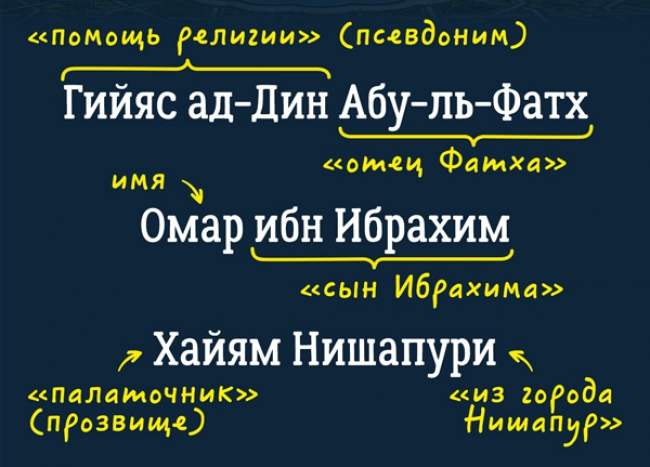
\includegraphics[width=0.7\linewidth]{img/haiyam}
    \caption{Расшифровка полного имени \emph{Омара Хайяма}}
    \label{fig:haiyam}
\end{figure}

\section{Китайские имена}

\section{Тибетские имена}

Тибетская система им\"eн принципиально отличается от китайской и ориентирована в большей степени на Индию. В Тибете нет фамилий. Многие имена являются калькой с санскрита, но есть и традиционные (напр.: \emph{Дава} (тиб. \emph{луна, понедельник}), \emph{Ньима} (тиб. \emph{солнце, воскресенье})).

\emph{Джамьянг Шэпа} -- тибетский уч\"eный.

\section{Корейские имена}

Корейское имя состоит из фамилии и следующего после него личного имени.

В большинстве случаев фамилия состоит из одного слога, а имя из двух слогов. Как имя, так и фамилия часто записываются с помощью \emph{ханча} -- китайских иероглифов, отражающих корейское произношение. Ханча более не используются в Северной Корее, а их использование для имён в Южной Корее сокращено до 5038 иероглифов. При использовании европейских языков некоторые корейцы сохраняют традиционный порядок написания, а другие меняют его согласно западной схеме.

В Корее используется всего около 250 фамилий. Самыми распространёнными из них являются \emph{Ким}, \emph{Ли} и \emph{Пак}. Однако большинство однофамильцев не являются близкими родственниками. Происхождение корейских фамилий тесно связано с корейской историей и географией.

\emph{Ким Дон Ин} -- корейский писатель.

\emph{Ким Юджон} -- корейский писатель.

\emph{Пак Кю Су} -- корейский государственный деятель и писатель.

% TODO Японские имена

% TODO Индийские имена

\section{VIAF}

Для выяснения форм написания имени и фамилии рекомендуется использовать сайт \underline{http://viaf.org} (англ. \emph{Virtual International Authority File} — виртуальный международный авторитетный файл) -- виртуальный каталог международного нормативного контроля (информации о произведениях и их авторах). В разработке проекта участвовало несколько крупнейших мировых библиотек, в том числе Немецкая национальная библиотека, Библиотека Конгресса США и РНБ.

\begin{figure}
    \centering
    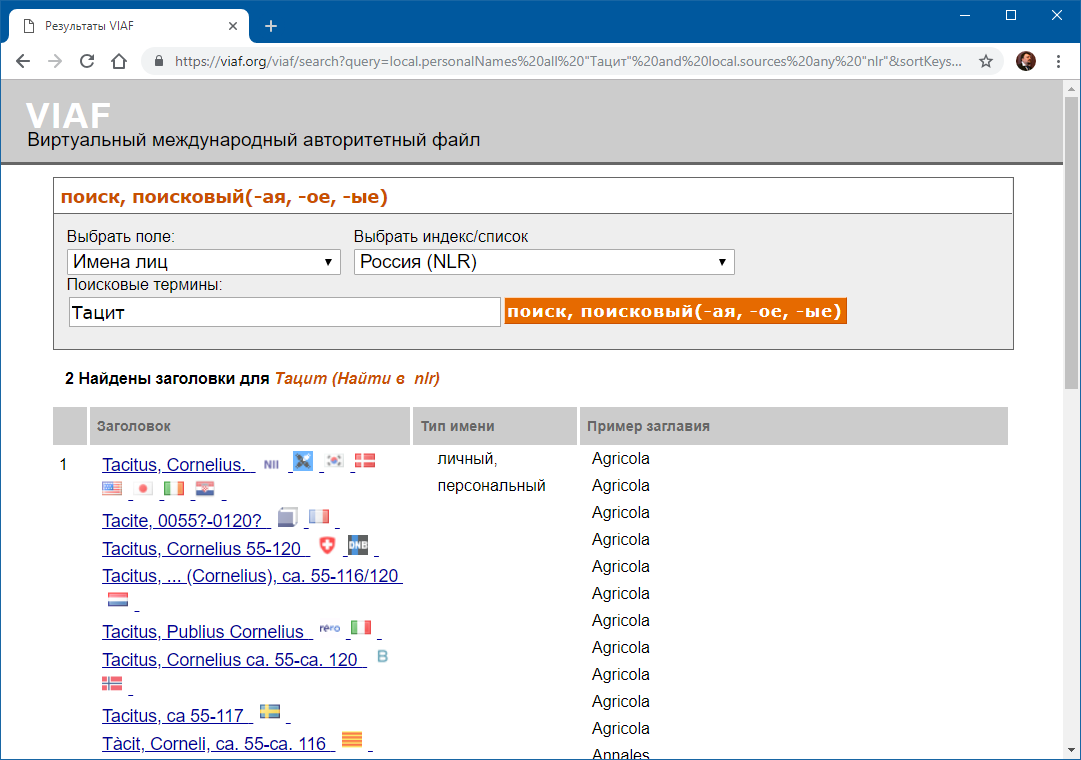
\includegraphics[width=\linewidth]{img/viaf}
    \caption{Сайт VIAF}
    \label{fig:viaf}
\end{figure}
